Условие задачи: Построить фазовый портрет системы дифференциальных уравнений 

$$
\left\{\begin{matrix}
 \frac{dx}{dt} = -y - x * (x^{2} + y^{2} - 1) \\
 \frac{dy}{dt} = x - y * (x^{2} + y^{2} - 1)
\end{matrix}\right
$$

Решение задачи (листинг):

\begin{minted}{python}
import numpy as np
from scipy.integrate import solve_ivp
import matplotlib.pyplot as plt

# Определение системы уравнений
def system(t, z):
    x, y = z
    dxdt = -y - x * (x**2 + y**2 - 1)
    dydt = x - y * (x**2 + y**2 - 1)
    return [dxdt, dydt]

# Сетка значений для построения фазового портрета
x = np.linspace(-2, 2, 20)
y = np.linspace(-2, 2, 20)
X, Y = np.meshgrid(x, y)

# Вычисление направлений векторного поля
U = -Y - X * (X**2 + Y**2 - 1)
V = X - Y * (X**2 + Y**2 - 1)

# Нормализация векторов для корректного отображения направлений
magnitude = np.sqrt(U**2 + V**2)
U /= magnitude
V /= magnitude

# Построение фазового портрета
plt.figure(figsize=(10, 8))
plt.quiver(X, Y, U, V, color="blue", alpha=0.8)
plt.title("Фазовый портрет системы", fontsize=14)
plt.xlabel("x", fontsize=12)
plt.ylabel("y", fontsize=12)
plt.axhline(0, color='black', linewidth=0.8, linestyle='--')
plt.axvline(0, color='black', linewidth=0.8, linestyle='--')
plt.grid()
plt.show()
\end{minted}

Вывод:

\begin{figure}[h]
    \centering
    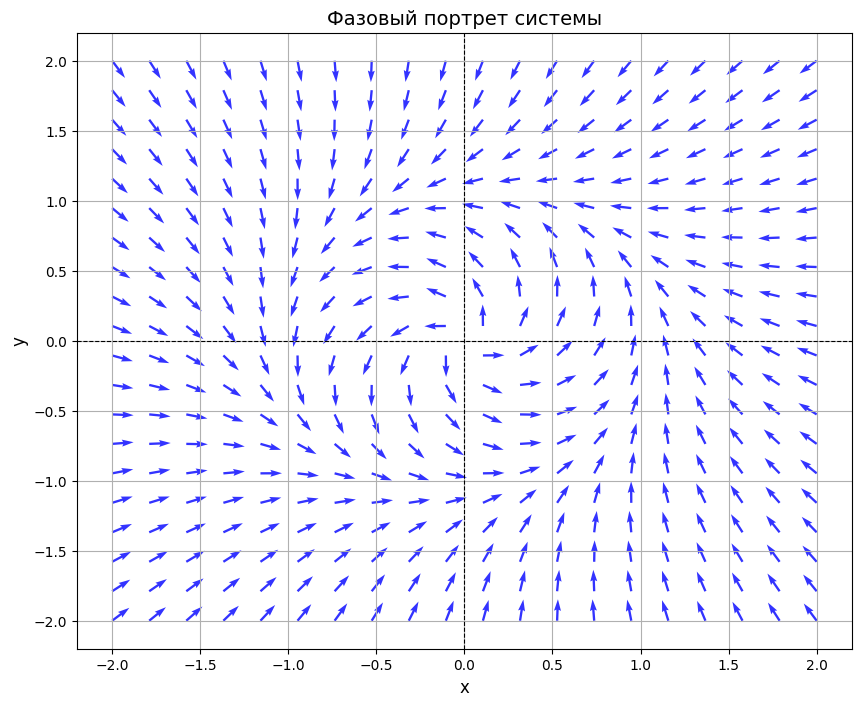
\includegraphics[width=0.8\linewidth]{pics/task2_result.png}
    \caption{Результат работы программы}
    \label{fig:mpr}
\end{figure}